\section{Modelo de Banco de Dados} \label{ModelagemBD} % ### 5.4. Modelo de Banco de Dados

Considerando as informações necessárias para o presente trabalho, e também o preparo de campo para potenciais aplicações futuras, foi elaborado um diagrama conceitual de banco de dados, que pode ser visto na Figura \ref{fig:DiagramConceitual}.

\begin{figure}[htbp]\centering
  \caption{\label{fig:DiagramConceitual} Diagrama Conceitual do banco de dados}
  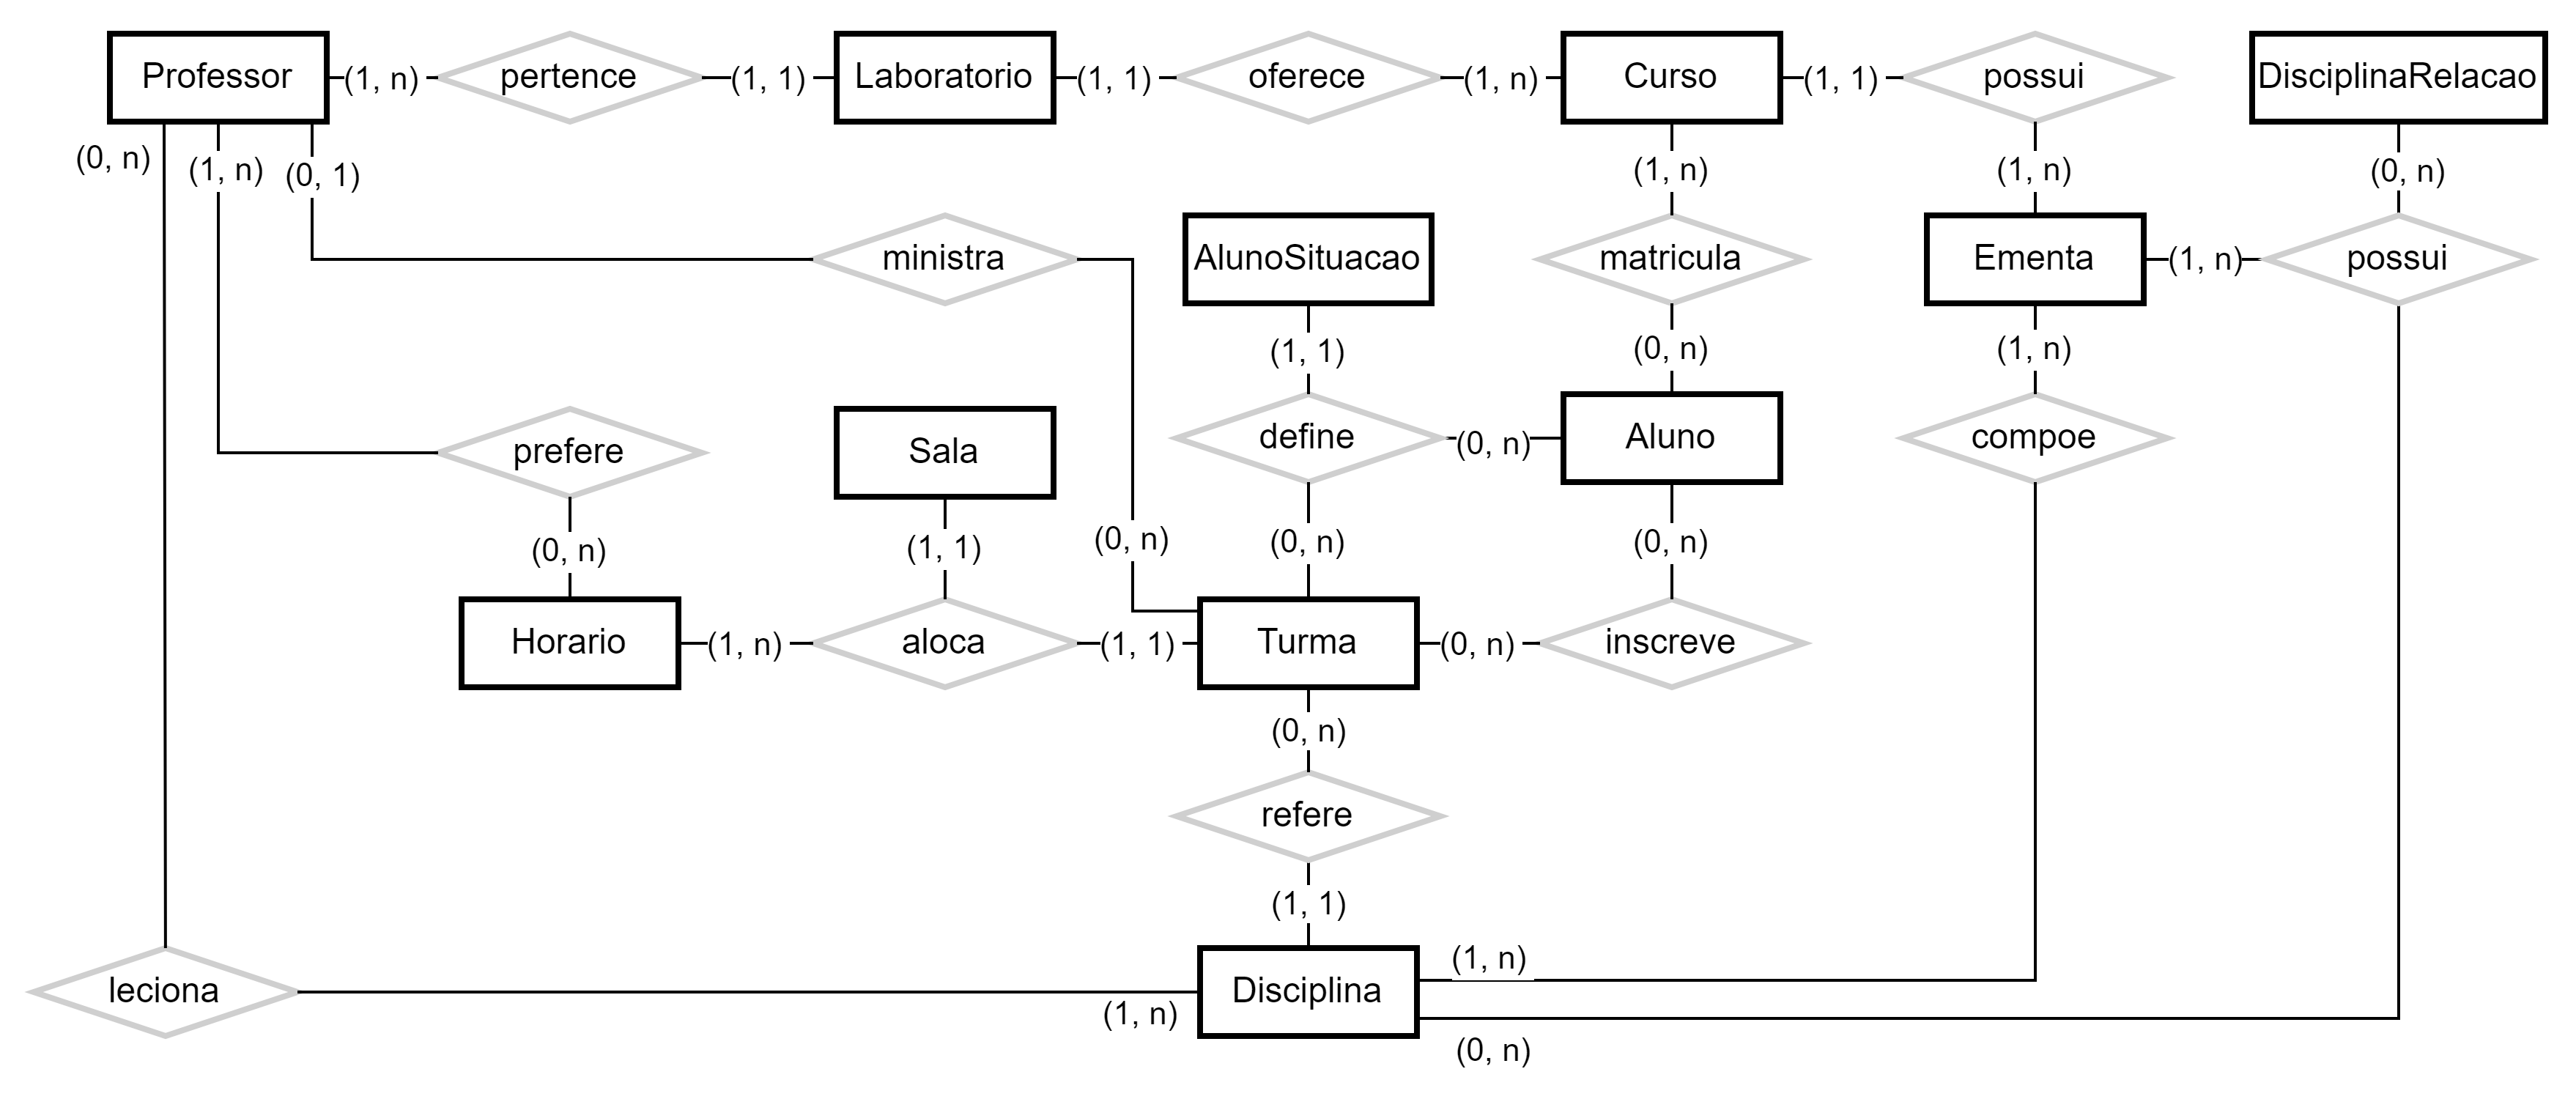
\includegraphics[scale=0.2]{files/img/DiagramaConceitual/DiagramaConceitualBranco.png}
  \legend{Fonte: o autor}
\end{figure} % Diagrama Conceitual

O diagrama conceitual foi elaborado utilizando a ferramenta \href{https://www.drawio.com/}{draw.io} citada na metodologia e ilustra as relações entre diversas entidades presentes na realidade da UENF. O emaranhamento presente no diagrama ilustra a complexidade envolvida na criação de uma grade horária, onde diversas entidades se relacionam entre si.

Como principais apontamentos, podemos citar a parte principal do modelo que é a alocação de turmas. Ela, como já descrito, envolve a correlação entre alunos de diferentes cursos, professores, disciplinas, salas e horários. Além disso, também é possível notar a presença de entidades que não são diretamente relacionadas à alocação de turmas, mas que podem se mostrar úteis, como a relação entre professores e laboratórios, e a de disciplinas e ementas.

Embora o diagrama apresente uma visão mais completa de todas as interconexões possíveis, é importante ressaltar que o presente trabalho foca primordialmente na alocação das turmas para o curso de Ciência da Computação, e que a implementação do banco de dados será feita de forma a atender a essas necessidades, fazendo então uso de uma parte do diagrama conceitual.

% Tendo isso em vista, o modelo conceitual reduzido para o presente trabalho pode ser visto na Figura \ref{fig:DiagramConceitualReduzido}.

% \begin{figure}[htbp]\centering
%   \caption{\label{fig:DiagramConceitualReduzido} Diagrama Conceitual reduzido para o presente trabalho}
%   \includegraphics[scale=0.2]{files/img/DiagramaConceitual/DiagramaConceitualReduzidoBranco.png}
%   \legend{Fonte: o autor}
% \end{figure} % Diagrama Conceitual reduzido

Neste modelo, mais enxuto, temos apenas as entidades principais, onde temos uma turma de determinada disciplina, ministrada por um professor e que ocorre em uma sala em um determinado horário.

\subsection{Diagrama de Entidade e relacionamento} % ### 5.4.1. Modelo Relacional

% Com isso, restamos o diagrama de Entidade e Relacionamento (DER) que pode ser visto na Figura \ref{fig:DER}.

% \begin{figure}[htbp]\centering
%   \caption{\label{fig:DER} Diagrama de Entidade e Relacionamento}
%   \includegraphics[scale=0.2]{files/img/DER/DERBranco.png}
%   \legend{Fonte: o autor}
% \end{figure} % Diagrama de Entidade e Relacionamento

Neste diagrama vemos as entidades principais, que são \textit{Turmas}, \textit{Disciplinas}, \textit{Professores}, \textit{Horários} e \textit{Salas}. As propriedades escolhidas para cada entidade são compostas por uma mistura de critérios. Por exemplo, o nome do professor, o código da disciplina, e a junção de código e bloco auxiliam primordialmente na identificação real dos professores, disciplinas e salas. Já as informações ``período'', ``apelido'' e ``comment''...

E também é notável a presença da entidade \textit{Alunos}, que se apresenta desacoplado das demais entidades. O motivo para isso é que, embora os alunos façam parte do processo de alocação de turmas, ao longo do desenvolvimento, o desenvolvimento de funcionalidades envolvendo os alunos...

\section{História do desenvolvimento} % ### 5.5.1. História do desenvolvimento

%% Acho que vai ficar mais fácil assim

Após a elaboração dos protótipos com o Figma, e da conceitualização diagramática do banco de dados, o desenvolvimento do sistema foi iniciado. Por maior familiaridade com a linguagem e considerando que é uma das mais utilizadas no mercado para desenvolvimento web [buscar referência], foi escolhida a linguagem JavaScript, utilizando a biblioteca React para a criação dos componentes visuais, ou seja, o front-end, e o Node.js para a criação do back-end e a criação de um servidor local que permitiria visualizar as mudanças no código em tempo real.

% Perguntar pra quem sabe, sobre qual é o real papel do Node.js

\subsection{Primeira versão} % ### 5.5.2. Primeira versão

A primeira versão do sistema foi desenvolvida em um ambiente local, com o objetivo de se aproximar ao máximo das páginas previstas no protótipo. Para isso, foi utilizada a biblioteca React Router para a navegação entre as páginas, e a biblioteca React Select para as caixas de seleção.

\subsubsection{Banco de Dados primitivo}

Os dados contidos no sistema foram inicialmente armazenados em arquivos JSON, que eram importados diretamente para o código. Isso foi feito para que fosse possível visualizar o funcionamento do sistema sem a necessidade de um banco de dados real. A partir disso, foi possível visualizar o funcionamento do sistema e realizar testes de usabilidade. Em contrapartida, os dados disponíveis não eram modificáveis, tendo apenas a possibilidade de leitura e mutação temporária, visto que após recarregar ou mudar de página, as mudanças eram perdidas.

Nesse método, cada entidade era armazenada em um arquivo JSON separado, contendo esse um array de objetos, onde em cada objeto haviam as chaves, representando as propriedades da entidade, e os valores, representando os dados da entidade.

Como nesta dinâmica não havia uma forte correlação entre os dados, o frontend acabava sendo o responsável por unir todas as informações. Assim, por exemplo, para se obter a lista de professores de uma turma, era necessário importar todos os professores, todas as turmas, e então, a partir do nome do professor alocado àquela turma, buscar na listagem dos professores qual era o professor que correspondia àquele nome, para então agregar as informações.

\subsubsection{Funcionalidades iniciais}

Nessa primeira versão, algumas funcionalidades já começaram a ser esboçadas, principalmente as funcionalidades CRUD (Create, Read, Update, Delete) para as entidades principais do sistema. Embora, como já dito, os dados não fossem persistentes, foi possível visualizar o funcionamento das funcionalidades de criação e leitura de turmas, professores, disciplinas, salas e horários.

Nessa versão, também foi implementada uma checagem bruta de conflitos por alocação simultânea de professores em mais de uma turma e a checagem da quantidade de demanda de alunos em relação à capacidade das salas. Uma descrição mais detalhada das funcionalidades de conflitos está presente \hyperref[Conflitos]{adiante}.

Além dessas funcionalidades que se mantiveram até a conclusão do sistema, também foram desenvolvidas funcionalidades que não obtiveram o mesmo êxito e que foram deixadas de lado ao decorrer do caminhar. Dentre elas, podemos citar a definição de níveis de preferência de horários para professores, a definição das características especiais das salas, e o andamento dos alunos em relação às disciplinas. Houveram também outras que nem chegaram a ser desenvolvidas, como a realocação de turmas através de um sistema de arrastar e soltar e o uso de heurísticas para a realocação de turmas.

\subsubsection{GitHub Pages}

Após o desenvolvimento local, como forma de viabilizar o acesso ao sistema por parte de outros usuários, foi feito o \textit{deploy}, ou seja, foi feito o upload do sistema para um servidor online. Para isso, foi utilizado o serviço GitHub Pages que, por ser gratuito e de fácil utilização, foi a escolha mais adequada para o momento. O sistema pode ser acessado através do link \url{https://jvfd3.github.io/timetabling-UENF/}.

\subsection{Segunda versão} % ### 5.5.3. Segunda versão

Utilizando do feedback quanto aos resultados entregues na primeira versão, alguns pontos de melhoria foram identificados, sendo um deles, e o mais importante: o planejamento. Na primeira abordagem, o desenvolvimento foi feito seguindo notas e ideias soltas, sem um planejamento prévio, o que resultou em um sistema que, embora funcional, não atendia a todas as necessidades propostas. E ia além: exibia funcionalidades que não eram de todo necessárias, ou melhor dizendo, têm menor prioridade do que muitas outras.

% Mesmo com esta nova dinâmica, outras funcionalidades foram deixadas de lado. Uma das que foram deixadas de lado foi a possibilidade de fixar certas informações. A proposta era que, certas disciplinas como Cálculo e Álgebra que são ofertadas para múltiplos cursos, pudessem ser fixadas em horários específicos, para que simplificasse aos coordenadores dos cursos a alocação de turmas.

\subsubsection{GitHub Projects}

Com isso, utilizando o GitHub Projects, foi organizado uma tabela de tarefas, onde foram unificadas as diversas anotações e ideias, antes soltas. A partir disso, foi possível visualizar o que era mais importante e o que poderia ser deixado de lado.

% [ADICIONAR IMAGEM DA TABELA BONITINHA: https://github.com/users/jvfd3/projects/3]

Tendo este novo sistema de tarefas em prática, foi possível tranquilizar a mente quanto ao conflito entre as funcionalidades que precisavam ser desenvolvidas, as que já estavam prontas, as que poderiam ter melhorias e quais se desejava implementar no futuro.

As tarefas foram inicialmente divididas em três principais categorias: \textit{Status}, \textit{Pages} e \textit{Sequence}. O \textit{Status} reflete o andamento da tarefa, se ela está disponível, em andamento, ou concluída. O \textit{Pages} reflete em qual página do sistema a tarefa se encontra, e o \textit{Sequence} reflete a ordem de prioridade da tarefa.

\subsubsection{Permanência dos dados}

Tendo agora uma rota mais clara a ser seguida, o desenvolvimento foi retomado. Uma das características mais marcantes e ainda não atribuídas ao sistema era a manutenção dos dados. Para exemplificar o funcionamento geral da permanência dos dados, consideremos o uso de uma \textit{REST API} utilizando de 4 ``camadas'': A. o frontend; B. os endpoints; C. as funções de execução; D. o banco de dados.

% [Usar diagrama para ilustrar]

O \textbf{frontend} é a interface do sistema, onde o usuário interage com o sistema. Ele se encontra em duas formas: a primeira é o chamado ``em produção'', que é o sistema que o usuário final acessa, e a segunda é o chamado ``em desenvolvimento'', que é o sistema que o desenvolvedor acessa para realizar as modificações necessárias. Ambas precisam se comunicar com o backend para realizar as quatro operações básicas no banco de dados (criação, leitura, atualização e deleção) por sobre as entidades existentes (turmas, professores, disciplinas, salas, etc.). Elas assim o fazer ao enviar requisições HTTP (GET, POST, PUT e DELETE), contendo pacotes de informações em formato JSON para os \textbf{endpoints}.

Os \textbf{endpoints} são as rotas que o backend disponibiliza para a recepção das requisições HTTP. Eles são responsáveis por encaminhar as requisições recebidas. Se funcionamento é simples: rotear as requisições recebidas junto com sua carga útil. Para tanto, as rotas criadas refletem diretamente a qual entidade do banco de dados a requisição se refere, sendo então assim sabido qual \textbf{função} deve ser executada.

As \textbf{funções} são as responsáveis por executar as operações no banco de dados. Elas processam o pacote de informações recebido, e então realizam a operação desejada no \textbf{banco de dados}.

O \textbf{banco de dados} recebe a requisição, processa a operação, e então retorna o status da operação. Esse retorno é então repassado camada por camada, até chegar ao frontend, onde o usuário final pode visualizar o resultado da operação.

\textbf{Resumidamente}: O \textbf{frontend} envia uma requisição HTTP com uma carga de informações a um \textbf{endpoint}, que encaminha a requisição a uma \textbf{função} específica que executa uma operação no \textbf{banco de dados}, assim retornando o status da operação ao frontend.

\paragraph*{\href{https://jsonbin.io/}{JSONBin}}

Como até então os dados estavam armazenados em formato JSON, imaginou-se que a melhor forma de persistir os dados seria através de um banco de dados que lidasse com JSON, e o escolhido foi o JSONBin.

Esta plataforma permite a criação de \textit{bins}, que são basicamente coleções de dados em formato JSON. A partir disso, é possível realizar requisições HTTP para a leitura, escrita, atualização e remoção dos dados. A utilização do JSONBin foi feita através de requisições HTTP usando o objeto \textit{XMLHttpRequest} do JavaScript, e a comunicação entre o frontend e o JSONBin foi feita através de \textit{tokens} de acesso.

Com isso, se tornou possível ler e atualizar os dados de forma remota, e assim, manter os dados mesmo após a recarga da página. Embora cumprisse com o que promete e o que era desejado, o JSONBin não se mostrou a melhor escolha para o sistema, visto que a sua utilização não performou tão bem quanto se esperava. Não se sabe se foi por inexperiência ou por limitações do próprio serviço, mas a utilização do JSONBin para a coleta dos dados, fazia com que a tela de carregamento do sistema demorasse alguns segundos para ser exibida, o que não é apropriado para a usabilidade do sistema proposto.

\paragraph*{MySQL}

Embora houvesse o desejo do uso de informações em formato JSON, achou-se por bem utilizar um banco de dados mais usual, recorrendo então ao MySQL, sendo então necessário criar um banco de dados local que armazenasse os dados e que pudesse ser acessado pelo sistema. Essa configuração serviu para estabelecer a supracitada camada de Banco de Dados. E consistiu basicamente na instalação do MySQL Server.

\subparagraph*{Migração dos dados}

Como os dados se encontravam em formato JSON, primariamente utilizou-se da ferramenta de importação de dados do próprio \textbf{MySQL Workbench}. Durante essa importação, o software automaticamente identifica os campos, criando a tabela e suas colunas. Porém, devido à quantidade dos dados, essa importação tendia a ser demorada, e por vezes, falhava, sem haver uma explicação clara do porquê.

Com isso, foi necessário recorrer a uma abordagem semimanual, sendo então desenvolvido um código em Python que lê os arquivos JSON e os converte em arquivos SQL para que as queries pudessem ser executadas no MySQL Workbench. A partir disso, foi possível importar os dados de forma mais rápida e eficiente.

Apesar da primeira tentativa de importação não ter sido completamente bem sucedida, foi desta forma que as tabelas foram inicialmente criadas. Não seguindo objetivamente a \hyperref[ModelagemBD]{modelagem anteriormente citada}. Isso gerou posteriormente a necessidade de ajustes manuais, como a adição de chaves primárias e estrangeiras, e a alteração de tipos de dados. Porém, como neste momento, o sistema visava apenas replicar o funcionamento do JSONBin, essas alterações não foram feitas de imediato.

\subparagraph*{Acesso ao Banco de Dados}

Seguindo a mesma sequência de camadas, o acesso ao banco de dados continua sendo feito através de requisições HTTP, porém, ao invés de serem enviadas ao JSONBin, são enviadas a um servidor local que executa as operações no banco de dados.

No \textbf{frontend}, enquanto que para acessar a API já pronta do JSONBin foi utilizado o objeto \textit{XMLHttpRequest}, para a comunicação com o banco de dados local, foi utilizada a biblioteca \textit{Axios} para construir as requisições HTTP. E elas, ao invés de serem enviadas ao JSONBin, são enviadas ao \textbf{servidor local}.

Na criação deste \textbf{servidor local} utilizou-se a biblioteca \textit{Express} em um código que era executado à parte do sistema principal. Essa biblioteca é responsável por criar todas as rotas necessárias para a comunicação entre o frontend e o banco de dados. A partir disso, foi possível criar rotas para cada uma das entidades, e para cada uma das operações CRUD. Com isso, cada operação CRUD em cada uma das rodas é encaminhada para uma \textbf{função específica} que executa a operação no banco de dados.

Este uso, embora exemplifique a aplicação da permanência dos dados, ela está limitada por dois aspectos: em primeira instância, a permanência dos dados é limitada ao servidor local, não sendo este o desejo final do sistema. Em segunda instância, para haver o acesso aos dados, é necessário que, além do banco de dados, o backend também esteja em execução, entretanto, o GitHub Pages, onde o sistema está hospedado, não viabiliza essa execução. Com isso viu-se necessária a busca por um novo serviço de hospedagem.

\subsubsection{Amazon Web Services}

Para suprir a necessidade de um servidor que pudesse executar o backend do sistema em conjunto com o banco de dados, foi escolhido o Amazon Web Services (AWS). O AWS é um serviço de computação em nuvem que oferece uma ampla gama de serviços, entretanto, apenas alguns deles foram necessários para o sistema.

O uso da AWS segue a mesma lógica do servidor local, com a diferença de que o servidor está em nuvem, e não localmente, assim resolvendo um dos dois problemas citados. Neste contexto, o uso da AWS foi feito através de três serviços principais: o \textit{API Gateway} para a recepção das requisições HTTP, o \textit{Lambda Functions} para a execução das funções que acessam o banco de dados, e o \textit{RDS} para o armazenamento dos dados; serviços estes que serão descritos mais detalhadamente a seguir.

O uso desses três serviços permitiu a execução do backend do sistema em nuvem, e assim, atingindo a permanência dos dados. Com isso, o sistema passou a ser capaz de manter os dados mesmo após a recarga da página, e assim, atender a uma das principais necessidades do sistema.

% \paragraph*{CORS} % Até agora não entendi direito pra que serve isso.

\paragraph*{Implantação}

O conjunto de funcionalidades da AWS envolve em grande parte o objetivo de manter um sistema constantemente acessível através da internet, ainda assim, durante o desenvolvimento, ou até mesmo durante o ciclo de vida do software, é esperado que ocorram manutenções períodicas nas quais é compreensível que o sistema fique fora do ar. Sendo assim, para manter-se visando ao máximo a acessibilidade do sistema, espera-se que o mesmo fique desconectado o mínimo possível.

Tanto o API Gateway quanto as funções Lambda precisaram sofrer diversas modificações ao longo do desenvolvimento, e para que essas modificações fossem aplicadas. A aplicação dessas modificações é chamada de implantação (\textit{deploy}), onde a AWS substitui a versão atual do sistema pela nova versão. Essa aplicação de modificações foi inicialmente feita através da interface web da AWS, porém, com o tempo, foi percebido que essa abordagem era ineficiente. No caso do API Gateway, a ineficiência não era tão grande, visto que assim que as rotas estiverem configuradas, não há a necessidade de alterá-las. Já no caso das funções Lambda, cada mínima mudança no código requisitava um novo deploy para cada uma das funções alteradas.

Outro detalhe percebido, foi que boa parte do código se repetia entre as funções que interagiam diretamente com o banco de dados. Sendo assim, passou-se a utilizar das Lambda Layers, que são camadas que podem ser compartilhadas entre diversas funções, e assim, diminuir a quantidade de código repetido. Essa nova abordagem permitiu que as funções fossem mais enxutas, e que as mudanças fossem aplicadas de forma mais rápida, visto que bibliotecas e funções comuns entre as funções eram compartilhadas entre elas.

\paragraph*{AWS CLI}

Nas primeiras tentativas de deploy, duas abordagens eram utilizadas: a primeira era a de copiar e colar o código diretamente na interface web da AWS, e a segunda era a de fazer o upload de um arquivo zip contendo o código. No segundo código, o código de deploy se assemelha ao seguinte.

\begin{lstlisting}[caption={Código de deploy de Lambda},label={lst:lambda}]
aws lambda create-function \
--function-name createProfessor \
--runtime nodejs20.x \
--role arn:aws:iam::375423677214:role/LambdaRole \
--handler index.handler \
--zip-file fileb://Files/AWS/lambdas/createProfessor/createProfessor.zip \
\end{lstlisting}

Como mostrado no Código \ref{lst:lambda}, usa-se o software AWS CLI para criar uma função lambda. O comando \textit{create-function} é o comando que cria a função, e os argumentos que seguem são os parâmetros necessários para a criação da função. O \textit{function-name} é o nome da função, o \textit{runtime} é a versão do Node.js que a função utiliza, o \textit{role} é o conjunto de permissões criadas na seção AWS Identity and Access Management (IAM), o \textit{handler} é o nome do arquivo principal que contém a função, e o \textit{zip-file} é o arquivo zip que contém o código da função.

Com isso, ao executar o comando, a função é criada, e então, a nova versão do código é aplicada. Com este fluxo de trabalho, embora permita o deploy sem a direta conexão ao sistema AWS, ainda assim é necessário executar comandos específicos para cada uma, tendo que manualmente compactar o código e fazer o upload de cada um dos arquivos das diversas funções coexistentes.

\paragraph*{SAM}

Como solução, foi utilizado o AWS SAM (Serverless Application Model), que é uma extensão do AWS CloudFormation que simplifica o desenvolvimento de aplicações sem servidor. O AWS SAM permite a definição de aplicações sem servidor de forma mais simples, e a partir disso, é possível fazer o deploy de toda a aplicação de uma vez só. O uso do AWS SAM foi feito através de um arquivo \textit{template.yaml}, que contém a definição de todas as funções Lambda, e de recursos necessários para o funcionamento do sistema.

\begin{lstlisting}[caption={Exemplo de template.yaml},label={lst:template}]
AWSTemplateFormatVersion: "2010-09-09"
Transform: AWS::Serverless-2016-10-31
Description: "OurClass>SAM>General>"

Resources:
  # LAYERS
  dbFunctionLayer:
    Type: AWS::Serverless::LayerVersion
    Properties:
      LayerName: dbFunctionSAM
      Description: connect to db
      ContentUri: ./layers/dbConnection
      CompatibleRuntimes:
        - nodejs14.x
        - nodejs16.x
        - nodejs18.x
  # API GATEWAY
  TimetablingAPI:
    Type: AWS::Serverless::Api
    Properties:
      StageName: timetablingStage
      EndpointConfiguration: REGIONAL
      Cors:
        AllowMethods: "'GET,POST,PUT,DELETE,OPTIONS'"
        AllowHeaders: "'Content-Type,X-Amz-Date,Authorization,X-Api-Key,X-Amz-Security-Token'"
        AllowOrigin: "'*'"

  # LAMBDA FUNCTIONS
  createProfessor:
    Type: AWS::Serverless::Function
    Properties:
      FunctionName: createProfessor
      CodeUri: ./lambdas/professor/createProfessor
      Events:
        ApiEvent:
          Type: Api
          Properties:
            Path: /professor
            Method: post
            RestApiId: !Ref TimetablingAPI
      Runtime: nodejs14.x
      Handler: index.handler
      Role:
        Fn::Sub: arn:aws:iam::${AWS::AccountId}:role/LambdaRole
      Layers:
        - !Ref dbFunctionLayer
      Environment:
        Variables:
          DB_HOST: ourclassuirds.cgsgwtemx5r8.us-east-2.rds.amazonaws.com
          DB_NAME: OurClassDB
          DB_USER: tang
          DB_PSWD: annabell
  readProfessor:
  # [...]
  updateProfessor:
  # [...]
  deleteClassTime:
  Type: AWS::Serverless::Function
  Properties:
    FunctionName: deleteClassTime
    CodeUri: ./lambdas/classTime/deleteClassTime
    Events:
      ApiEvent:
        Type: Api
        Properties:
          Path: /classTime/{id}
          Method: delete
          RestApiId: !Ref TimetablingAPI
    Runtime: nodejs14.x
    Handler: index.handler
    Role:
      Fn::Sub: arn:aws:iam::${AWS::AccountId}:role/LambdaRole
    Layers:
      - !Ref dbFunctionLayer
    Environment:
      Variables:
        DB_HOST: ourclassuirds.cgsgwtemx5r8.us-east-2.rds.amazonaws.com
        DB_NAME: OurClassDB
        DB_USER: tang
        DB_PSWD: annabell
\end{lstlisting}

Como mostrado no Código \ref{lst:template}, o arquivo \textit{template.yaml} contém a definição de algumas das estruturas utilizadas para este sistema, principalmente as funções Lambda, visto que são quatro funções para cada uma das seis entidades, totalizando 24 funções. O arquivo contém a definição de cada uma das funções, e de cada uma das rotas que elas atendem. A partir disso, é possível fazer o deploy de todas as funções que foram alteradas de uma vez só, e assim, diminuir o tempo de deploy e a quantidade de comandos necessários.

Após o preparativo do arquivo \textit{template.yaml}, o deploy é feito através do conjunto de comandos \textit{sam build; sam deploy}, que primeiro combina o \textit{CloudFormation Template} com o código da aplicação, e em seguida realiza o deploy de todas as funções definidas no arquivo. Com isso, o sistema passou a ser mais facilmente atualizável, e mais facilmente mantido.

\subsubsection{Funcionalidades adicionais}

Acrescendo à visualização de conflitos desenvolvida na primeira versão, foi implementada a visualização de conflito por capacidade de salas, ao comparar com a quantidade de alunos estimados para a turma. Mais detalhes sobre os conflitos podem ser vistos mais adiante na \hyperref[Conflitos]{seção de conflitos}.

Adicionou-se também diversas filtragens, principalmente na página de \textbf{Grade Horária}. Dessa forma, torna-se possível a visualização específica de turmas que atendam a certos critérios. Essa filtragem é feita através de caixas de seleção, onde é possível selecionar quais critérios se deseja filtrar, sendo eles: ano, semestre, categoria, disciplina, professor e sala. Essa coletânea de filtros viabiliza uma análise mais limpa das informações estruturadas, podendo então gerar \textit{insights} quanto ao posicionamento histórico das turmas.

Outra utilidade adicionada, agora na página \textbf{MultiTurmas}, foi a seção de ``Disciplinas ainda não oferecidas''. Sua funcionalidade consiste em dispor ao usuário uma lista de disciplinas que, segundo a ementa de Ciência da Computação, deveriam ser ofertadas naquele semestre. A partir disso, o usuário pode então selecionar o botão correspondente àquela disciplina e, a partir disso, uma turma para esta disciplina é adicionada à lista de turmas ofertadas. Há também um botão no topo que permite a adição de todas as disciplinas de uma vez.

\subsection{Terceira versão} % ### 5.5.3. Terceira versão % https://github.com/jvfd3/timetabling-UENF/issues/348

% Na programação como um todo, é comum que se busquem padrões durante o desenvolvimento, incluindo, mas não se limitando a, padrões

Considerando que a segunda versão já apresentava em sua maioria as funcionalidades mínimas desejadas, a terceira versão foi focada em melhorias de usabilidade e na correção de bugs.

- Nova estrutura no GitHub Projects
-- Charts GitHub
- Layout de professor, disciplina, demanda e descrição de turma;
- Criação de turma por disciplina plus: solução inicial;
- Aumento na quantidade dados cadastrados;
- Adição de disciplinas e professores;
- Aprimoramento na forma de criação de itens: "usar os valores mudados anteriores como se fosse o novo item" vs "criar um novo item limpo"
- Diversas melhorias de boas práticas de programação
-- Repadronização de componentes
--- Migração de código para inglês
--- Padronização de cores de conflitos
-- Remoção de "ordem"
-- Cloudformation
- Salas pouco usuais;
- Aprimoramento dos ids identificadores dos conflitos
- Correção dos delays e criação e deleção de turmas e horários
-- Bug de deleção e criação sequenciais
- Separando disciplinas por categoria
-- Mostrar apenas turmas de CC por padrão

- Multiturmas:
1. Adição de filtros: disciplina, período esperado, professor, sala, categoria;
2. Adição de ordenações por: ano, semestre, disciplina período, disciplina nome, etc.;
3. Aprimoramento das labels dos selects.

- CCTable:
1. Ordenação por célula;
2. Aprimoramento das labels das células.

- CRUD (Turmas, Professores, Alunos, Salas, Disciplinas):
1. Omitir o item quando a seleção for nula

\section{Conflitos}\label{Conflitos} % ### 5.6. Conflitos

Uma das principais funcionalidades do sistema é a detecção de conflitos. Seu objetivo é auxiliar ao usuário a identificar possíveis problemas na alocação das turmas, e assim, permitir que ele possa corrigí-los antes de finalizar a grade horária. Diversas situações podem ser consideradas conflitos, e cada uma delas é tratada de forma diferente.

Deve-se ressaltar que o que aqui são chamados de conflitos, não são necessariamente o que são chamados de conflitos no contexto de programação linear. Aqui, conflitos são situações que podem ser consideradas inadequadas para a alocação de turmas, mas que ainda assim, não são completamente impeditivas para a alocação prática das turmas. Essa característica deve ser levada em consideração pois, apesar de geralmente retratar situações atípicas, é surpreendentemente recorrente a ocorrência de situações atípicas diversas.

\subsection{Típicos conflitos atípicos}

Para ilustração, abaixo estão descritos alguns exemplos de conflitos que poderiam ser alertadas pelo sistema, mas que não seriam realmente um restritor para a execução prática das alocações:

Considerando o diminuto corpo docente do curso de Ciência da Computação, que atualmente conta com seis professores doutores, é recorrente a solicitação de professores bolsistas para ministrar disciplinas. Devido aos prazos existentes ao longo do processo de criação da grade horária, é comum que ainda não se saibam quais e quantos professores bolsistas serão disponibilizados para quais turmas. Porém, como o Sistema Acadêmico requere a inserção de professores para a criação de turmas, uma solução encontrada foi a inserção de um desses professores permanentes como responsável pela turma. E, mesmo após se obter a informação quanto a quais e quantos bolsistas estarão disponíveis, ainda assim o sistema acadêmico não os permite serem inseridos, visto que eles não têm um vínculo permanente com a instituição. Com isso, seria possível ver, por exemplo, um conflito entre duas turmas que possuem o mesmo professor em um mesmo horário, mas que na prática, uma delas será ministrada por um professor bolsista.

Outras situações que podem ocorrer revolvem em torno da alocação das salas. Duas situações que podem ilustrar sua atipicidade são: a possibilidade de alocar uma turma a uma determinada sala, mesmo que se tenha a intenção de ministrá-la em outra, e também a possibilidade de se repartir a turma em duas salas de aula ocorrendo simultaneamente.

Esses e outros são exemplos de situações recorrentes ao longo do processo flexível da organização da tabela horária.

\subsection{Conflitos tratados pelo sistema}

Para a implementação, primeiro visou-se a detecção de conflitos que poderiam ser considerados restritores para a alocação das turmas. Sendo eles os de alocação simultânea de salas e professores, visto que um professor não pode ministrar duas turmas simultaneamente, nem uma sala deve comportar duas turmas simultaneamente (embora este segundo seja teoricamente possível).

Além disso, também foi implementada a detecção de conflitos de capacidade, onde a quantidade de alunos de uma turma é maior do que a capacidade da sala alocada, e alguns outros indicativos visuais que serão descritos abaixo.

Os conflitos calculados são representados de três formas diferentes. A primeira e mais perceptível é a mudança de cor de fundo das propriedades conflituosas. A segunda, visando evitar sobreposição de conflitos, é a adição de uma borda inferior que se estende por toda a largura da propriedade. E a terceira, mais descritiva, é o uso do atributo \textit{title} dos elementos HTML, que exibe uma mensagem de alerta flutuante ao passar o mouse sobre a propriedade conflituosa, assim dispondo de mais detalhes sobre os conflitos buscados e encontrados.

Embora o sistema seja projetado para ser permissivo quanto a inexistência de certas informações, é sempre esperado que a maior quantidade de informações possíveis seja inserida, assim, caso algum campo não tenha sido preenchido a cor de fundo do elemento será alterada para um tom acinzentado.

% "propriedades conflituosas" é um bom termo?

\subsubsection{Professores}

O sistema contempla a checagem de conflitos de alocação simultânea de professores em mais de uma turma. Ou seja, considerando todas as turmas ao qual o professor está atribuído no ano e semestre selecionados, o sistema compara todos os horários das turmas deste professor, e verifica se há alguma interseção entre horários que estão no mesmo dia, levando em conta a duração da aula.

Caso haja algum conflito, o sistema destaca o professor em questão, tornando a sua cor de fundo avermelhada. Além disso, ao passar o mouse sobre o nome do professor, é exibido um alerta flutuante, informando que quais são as turmas e horários que estão em conflito.

\subsubsection{Salas}

As salas também apresentam a verificação do conflito de alocação simultânea. Porém, diferente dos professores, a checagem é feita conferindo todos os horários na qual a sala está alocada, e então é feita a mesma verificação de interseção citada anteriormente. Havendo o conflito, é exibida uma borda alaranjada na parte inferior das propriedades referentes ao conflito, além de, assim como no caso dos professores, exibir o alerta flutuante.

Além disso, também é feita a comparação entre a quantidade máxima de alunos comportados na sala e a quantidade de alunos estimados para a turma. Este conflito por sua vez é ilustrado tornando avermelhado o fundo da demanda estimada e da seleção de salas. Caso uma turma tenha mais de um horário, é calculada a quantidade remanescente dos alunos que demandam a disciplina com relação a cada uma das capacidades das salas destes horários, mostrando cada um deles no alerta flutuante.

\subsubsection{Disciplina}

Além desses conflitos, outras características analisadas e representadas é quanto às disciplinas atribuídas às turmas, que, embora não representem necessariamente um \textit{conflito}, mas sim um indicativo, ainda assim serão tratatados como conflitos por motivos de simplificação. Esse indicativo leva em consideração o semestre selecionado e o período esperado da disciplina de certa turma. Utilizando de lógica similar, também é indicado caso não tenha sido atribuído um período à disciplina, e se, para o curso de Ciência da Computação, a disciplina é considerada como \textbf{Eletiva Livre}, \textbf{Eletiva Optativa}, ambas em tons azulados, ou se não é uma disciplina para o curso de Ciência da Computação, sendo então representada em tons alaranjados.

Os semestres possíveis são três: o primeiro semestre, o segundo semestre e o ``período de verão''. No caso do período de verão, as disciplinas que têm o seu período esperado neste semestre são marcadas com um tom amarelado, visto que não há relevância da sua paridade em um período de férias. Já nos casos das disciplinas de paridade ímpar (disciplinas dos períodos 1, 3, 5, 7 e 9) no primeiro semestre, ou as disciplinas de paridade par (disciplinas dos períodos 2, 4, 6, 8 e 10) no segundo semestre, estas são marcadas com um tom esverdeado, sendo aquelas referentes aos períodos finais do curso marcadas com um tom mais escuro. Já as disciplinas pares em semestres ímpares, ou as disciplinas ímpares em semestre pares, são ilustradas com a cor avermelhada, seguindo a mesma lógica de gradiente escuro nos últimos períodos.
